\documentclass{article}
\usepackage{amsmath}
\usepackage{hyperref}
\usepackage{graphicx}
\usepackage{adjustbox}
\newcommand{\tabincell}[2]{\begin{tabular}{@{}#1@{}}#2\end{tabular}}

\begin{document} %This is where document begins
\begin{titlepage}
\title{EE 232E \\Graphs and Network Flows\\Homework 1\\Winter 2016} 
\author{Liqiang Yu, Rongjing Bai, Yunwen Zhu\\
904592975, 204587519, 304588434}  %change your ID here
\date{04-12-2016}
\end{titlepage}

\maketitle
\newpage
\tableofcontents
\newpage

\section{Problem1}\label{prob:p1}
In this part, we create random networks with probability p for drawing an edge between two arbitrary vertices and discussion the relationship between p and connectedness of the graph.
\subsection{Part a}
(i) when p = 0.01, we can get the degree distribution in Figure \ref{fig:p1_1}.
\begin{figure}[htbp]
\centering
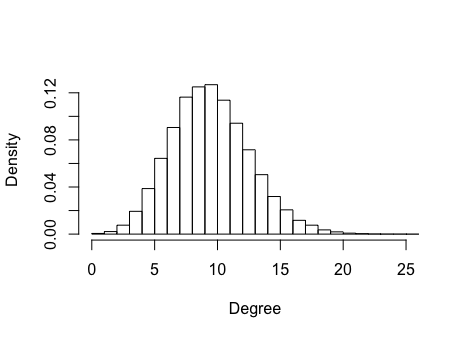
\includegraphics[width=.6\textwidth]{p1_1.png}
\caption{The degree distribution for p = 0.01}
\label{fig:p1_1}
\end{figure}\\
\\
(ii) when p = 0.05, we can get the degree distribution in Figure \ref{fig:p1_2}.
\begin{figure}[htbp]
\centering
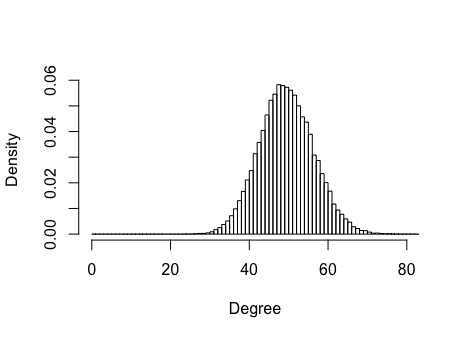
\includegraphics[width=.6\textwidth]{p1_2.png}
\caption{The degree distribution for p = 0.05}
\label{fig:p1_2}
\end{figure}\\
\\
(iii) when p = 0.1, we can get the degree distribution in Figure \ref{fig:p1_3}.
\begin{figure}[htbp]
\centering
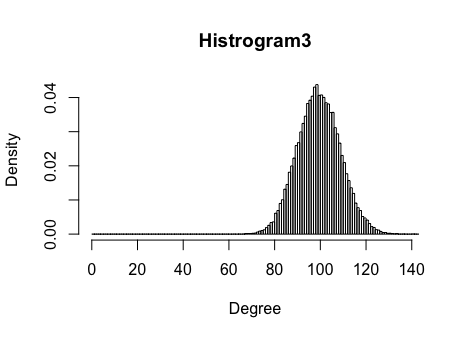
\includegraphics[width=.6\textwidth]{p1_3.png}
\caption{The degree distribution for p = 0.1}
\label{fig:p1_3}
\end{figure}\\
\\
Based on the three figures, we can see that as the probability for drawing an edge between two arbitrary vertices increases, the degree increases conrespondingly, which conforms to our thought. 
\subsection{Part b}
To check whether or not these network are connected and the diameter of these networks, we use is.connected() and diameter()function. And as this is the random network, we run the test for 50 times to get a more accurate result. Thus, in this way, we get the ratio of whether the network is connected and average diameter of the networks. The results are shown in Table \ref{tb:p1_b}.
\begin {table}[htbp]
\caption{parameters of random network}
\begin{adjustbox}{center}
\label{tb:p1_b}
\begin{tabular}{|c|c|c|c|}
\hline
\tabincell{c}{} & p = 0.01 & p = 0.05 & p = 0.1\\
\hline
\tabincell{c}{ratio of connectedness}&0.9&1&1\\
\hline
\tabincell{c}{diameter}&5.4&3&3\\
\hline
\end{tabular}
\end{adjustbox}
\end{table}\\
\\
Based on the results, we can see that the network has a rather high ration of connectedness. Thus, all of these networks can be regarded as connected.
\subsection{Part c}
In order to find out the value of $p_{c}$, we start from the small value of p until the network become connected. And as this is the random network, we run the test for 100 times to get a more accurate result. Thus, in this way, we get $p_{c}$ =  0.006371, which roughly corresponds to the value in theory.


\end{document}
